\begin{figure}[H]
    \centering
    \begin{subfigure}[t]{0.25\textwidth}
    \centering
    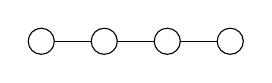
\begin{tikzpicture}[main node/.style={circle,draw}]
        % Vertexes
        \node[main node] (a) at ( 0, 0) {};
        \node[main node] (b) at ( 0.8, 0) {};
        \node[main node] (c) at ( 1.6, 0) {};
        \node[main node] (d) at ( 2.4, 0) {};
        % Edges
        \draw
            (a) edge (b)
            (b) edge (c)
            (c) edge (d);
        
    \end{tikzpicture} 
    
    \caption{}
    \label{img:classes:path}

    \end{subfigure}%
    \begin{subfigure}[t]{0.25\textwidth}
    \centering
    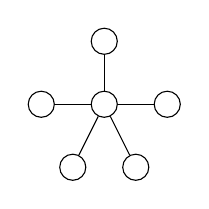
\begin{tikzpicture}[main node/.style={circle,draw}]
        % Vertexes
        \node[main node] (a) at (-0.8,    0) {};
        \node[main node] (b) at (   0,    0) {};
        \node[main node] (c) at ( 0.8,    0) {};
        \node[main node] (d) at (   0,  0.8) {};
        \node[main node] (e) at (-0.4, -0.8) {};
        \node[main node] (f) at ( 0.4, -0.8) {};

        % Edges
        \draw
            (b) edge (a)
            (b) edge (c)
            (b) edge (d)
            (b) edge (e)
            (b) edge (f);     

    \end{tikzpicture}  
    
    \caption{}
    \label{img:classes:star}

    \end{subfigure}%
    \begin{subfigure}[t]{0.25\textwidth}
    \centering
    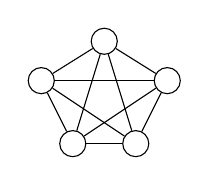
\begin{tikzpicture}[main node/.style={circle,draw}]
        % Vertexes
        \node[main node] (a) at (-0.8,    0) {};
        \node[main node] (b) at ( 0.8,    0) {};
        \node[main node] (c) at (   0,  0.5) {};
        \node[main node] (d) at (-0.4, -0.8) {};
        \node[main node] (e) at ( 0.4, -0.8) {};

        % Edges
        \draw
            (a) edge (b)
            (a) edge (c)
            (a) edge (d)
            (a) edge (e)

            (b) edge (c)
            (b) edge (d)
            (b) edge (e)

            (c) edge (d)
            (c) edge (e)

            (d) edge (e);     

    \end{tikzpicture} 

    \caption{}
    \label{img:classes:clique}

    \end{subfigure}%
    \begin{subfigure}[t]{0.25\textwidth}
    \centering
    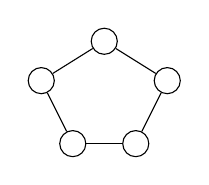
\begin{tikzpicture}[main node/.style={circle,draw}]
        % Vertexes
        \node[main node] (a) at (-0.8,    0) {};
        \node[main node] (b) at ( 0.8,    0) {};
        \node[main node] (c) at (   0,  0.5) {};
        \node[main node] (d) at (-0.4, -0.8) {};
        \node[main node] (e) at ( 0.4, -0.8) {};

        % Edges
        \draw
            (b) edge (c)
            (a) edge (d)
            (a) edge (c)
            (d) edge (e)
            (e) edge (b);     

    \end{tikzpicture} 

    \caption{}
    \label{img:classes:cycle}

    \end{subfigure}\\
    \begin{subfigure}[t]{0.25\textwidth}
    \centering
    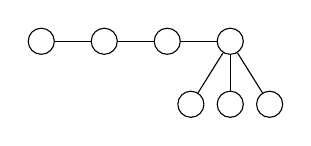
\begin{tikzpicture}[main node/.style={circle,draw}]
        % Vertexes
        %% Path
        \node[main node] (a) at ( 0, 0) {};
        \node[main node] (b) at ( 0.8, 0) {};
        \node[main node] (c) at ( 1.6, 0) {};
        \node[main node] (d) at ( 2.4, 0) {};
        
        %% Broom
        \node[main node] (e) at ( 1.9, -0.8) {};
        \node[main node] (f) at ( 2.4, -0.8) {};
        \node[main node] (g) at ( 2.9, -0.8) {};

        % Edges
        \draw
            (a) edge (b)
            (b) edge (c)
            (c) edge (d)
            (d) edge (e)
            (d) edge (f)
            (d) edge (g);

    \end{tikzpicture} 

    \caption{}
    \label{img:classes:broom}

    \end{subfigure}%
    \begin{subfigure}[t]{0.25\textwidth}
    \centering
    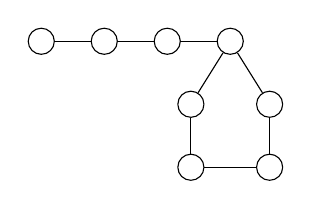
\begin{tikzpicture}[main node/.style={circle,draw}]
        % Vertexes
        %% Path
        \node[main node] (a) at ( 0, 0) {};
        \node[main node] (b) at ( 0.8, 0) {};
        \node[main node] (c) at ( 1.6, 0) {};
        \node[main node] (d) at ( 2.4, 0) {};
        
        %% Cycle
        \node[main node] (e) at ( 1.9, -0.8) {};
        \node[main node] (f) at ( 1.9, -1.6) {};
        \node[main node] (g) at ( 2.9, -0.8) {};
        \node[main node] (h) at ( 2.9, -1.6) {};

        % Edges
        \draw
            (a) edge (b)
            (b) edge (c)
            (c) edge (d)
            (d) edge (e)
            (d) edge (g)
            (e) edge (f)
            (f) edge (h)
            (h) edge (g);

    \end{tikzpicture} 

    \caption{}
    \label{img:classes:lollipop}

    \end{subfigure}%
    \begin{subfigure}[t]{0.25\textwidth}
    \centering
    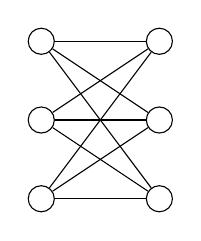
\begin{tikzpicture}[main node/.style={circle,draw}]
        % Vertexes
        %% Left
        \node[main node] (a) at ( -.5, 0) {};
        \node[main node] (b) at ( -.5, -1) {};
        \node[main node] (c) at ( -.5, -2) {};

        %% Right
        \node[main node] (d) at ( 1, 0) {};
        \node[main node] (e) at ( 1, -1) {};
        \node[main node] (f) at ( 1, -2) {};
        
        % Edges
        \draw
            (a) edge (d)
            (a) edge (e)
            (a) edge (f)

            (b) edge (d)
            (b) edge (e)
            (b) edge (f)

            (c) edge (d)
            (c) edge (e)
            (c) edge (f);

    \end{tikzpicture} 

    \caption{}
    \label{img:classes:compbip}

    \end{subfigure}%
    \begin{subfigure}[t]{0.25\textwidth}
    \centering
    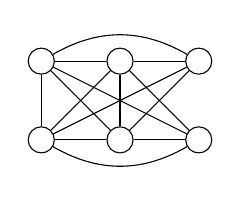
\begin{tikzpicture}[main node/.style={circle,draw}]
        % Vertexes
        %% Clique
        \node[main node] (a) at (-1, 0) {};
        \node[main node] (b) at (-1, 1) {};
        \node[main node] (c) at ( 0, 0) {};
        \node[main node] (d) at ( 0, 1) {};

        %% Independent Set
        \node[main node] (e) at ( 1, 0) {};
        \node[main node] (f) at ( 1, 1) {};

        % Edges
        \draw
            % Clique
            (a) edge (b)
            (a) edge (c)
            (a) edge (d)

            (b) edge (c)
            (b) edge (d)

            (c) edge (d)

            % Independent Set
            (e) edge[bend left] (a)
            (e) edge (b)
            (e) edge (c)
            (e) edge (d)

            (f) edge (a)
            (f) edge[bend right] (b)
            (f) edge (c)
            (f) edge (d);

    \end{tikzpicture} 

    \caption{}
    \label{img:classes:compsplit}

    \end{subfigure}

    \caption{Graphs representing graph classes related to efficient algorithms
    for token swap problems. Figure~\ref{img:classes:path} is a path of size
    4; Figure~\ref{img:classes:star} is a star; Figure~\ref{img:classes:clique}
    is a complete graph; Figure~\ref{img:classes:cycle} is a cycle; Figure~\ref
    {img:classes:broom} is a broom graph; Figure~\ref{img:classes:lollipop} is
    a lollipop graph; Figure~\ref{img:classes:compbip} is a complete bipartite
    graph; and Figure~\ref{img:classes:compsplit} is a complete split graph.}
    \label{img:classes}
\end{figure}